% Suggested figure for chapter 04_WindTurbineControl_02_notBold.tex: the bar plot
% (fig:EvalCrit1) and the Pareto plot (fig:CtrlCompAll) side by side in one figure.
% It replaces both figure environments (afig01_IPCMPCbar and afig01_IPCMPCpareto).
% The old labels are kept for the subfigures, so \ref{fig:EvalCrit1} and
% \ref{fig:CtrlCompAll} in the text still work (they then print e.g. 4.12a and 4.12b);
% fig:CtrlCompBarPareto refers to the whole figure.
% Note: inside the plots the rows are titled (a), (b), (c); the caption therefore
% calls them rows (top, middle, bottom).

\begin{figure}[htbp]
    \centering
    \subfloat[Bar plot\label{fig:EvalCrit1}]{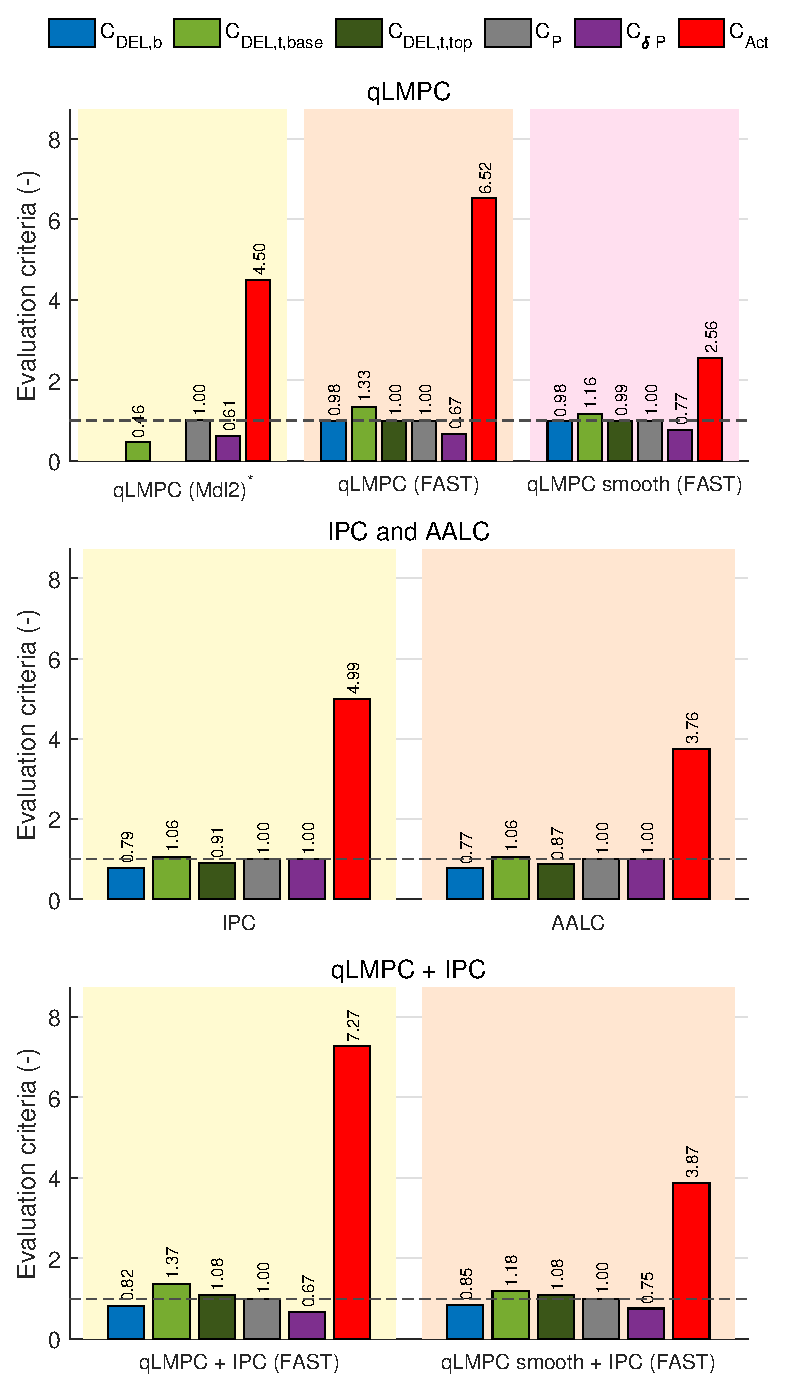
\includegraphics[width=0.49\textwidth]{figures/figures_WESC25/afig01_IPCMPCbar.eps}}\hfill
    \subfloat[Pareto plot\label{fig:CtrlCompAll}]{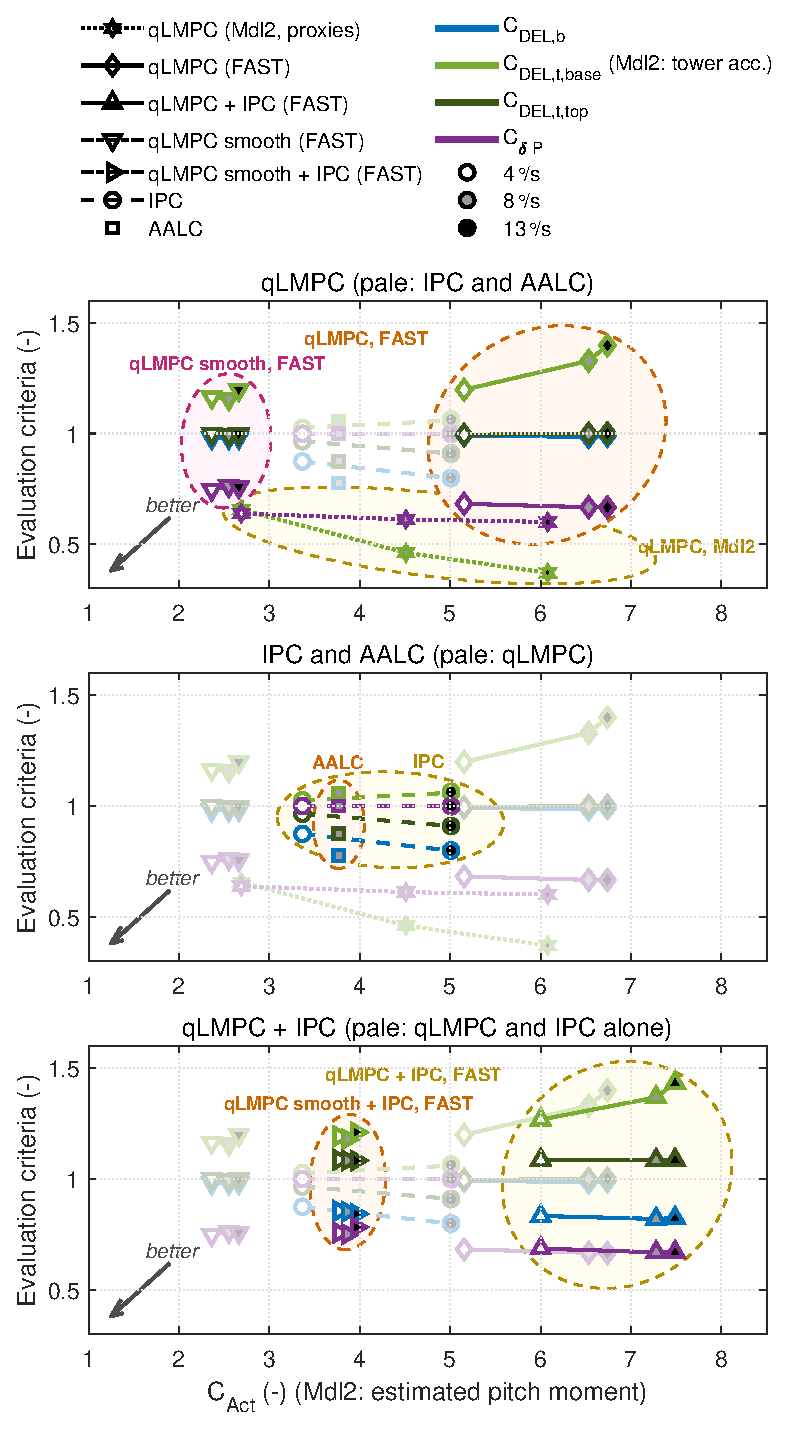
\includegraphics[width=0.49\textwidth]{figures/figures_WESC25/afig01_IPCMPCpareto.eps}}
    \caption[Evaluation criteria of qLMPC, IPC, and AALC for turbulent wind]{Evaluation criteria of the controllers for turbulent wind (18\,m/s mean, IEC turbulence class~B, second verification set), normalized by the PI baseline with the same pitch rate limit. Rows: qLMPC (top), IPC and AALC (middle), qLMPC combined with IPC (bottom). (a)~Bar plot at a pitch rate limit of 8\textdegree/s: blade DEL $C_{\mathrm{DEL},b}$, tower base and tower top DELs $C_{\mathrm{DEL},t,\mathrm{Base}}$ and $C_{\mathrm{DEL},t,\mathrm{Top}}$, mean power $C_{\bar{P}}$, power standard deviation $C_{\delta P}$, and actuator power $C_\text{Act}$. (b)~Pareto plot: $C_{\mathrm{DEL},b}$ (blue), $C_{\mathrm{DEL},t,\mathrm{Base}}$ (green), $C_{\mathrm{DEL},t,\mathrm{Top}}$ (dark green), and $C_{\delta P}$ (purple) over $C_\text{Act}$ for the pitch rate limits 4\textdegree/s (white markers), 8\textdegree/s (grey), and 13\textdegree/s (black); the controllers of the other rows are shown pale. The dashed ovals enclose all points of one controller; their colour matches the background of the same controller in the bar plot. $^*$qLMPC on Mdl2 (no model mismatch): tower top fore-aft acceleration instead of the tower base DEL, no blade and tower top DELs, $C_\text{Act}$ with the pitch moment estimated from a model fitted to FAST. The arrow points towards better results.}
    \label{fig:CtrlCompBarPareto}
\end{figure}
